\chapter{Overview}\label{sec:overview}

\section{Workflow Overview}

\cxoneflow has origins in CxFlow for the CxSAST product (CxSAST is the predecessor to \cxonens).  CxFlow
had a variety of functions and deployment options related to orchestrating scans in CxSAST and sending
result feedback to issue trackers.  \cxoneflow will also orchestrate scans but is adapted for the
concepts of \cxonens.

The \cxoneflow logic for how scans are orchestrated is very similar to that of CxFlow.  The basic
logic flow is that scans are executed when:

\begin{itemize}
    \item If a Push is made to a repository's protected branch, that protected branch is scanned.
    \item If a Pull Request is opened that targets a protected branch, a scan is performed on
    the source branch.
    \item If a Push is made to a branch that is the source of an open Pull Request that targets
    a protected branch, the open Pull Request branch is scanned.
\end{itemize}


\cxoneflow follows this workflow logic upon the receipt of a webhook event payload generated by the
source control management system (SCM). The code from the repository to be scanned is cloned by \cxoneflowns, 
collected into a zip file, then submitted for a scan to \cxonens.  When the scan is submitted,
the locally cloned code is deleted.


\section{Deployment Overview}

The method of deployment for \cxoneflow is intended to integrate scanning of all enterprise repositories
with a minimal amount of configuration.  The best method for deployment is to configure source control web
hooks where they will emit events for the largest possible number of repositories.  In many source control
systems, this can be done at a global or organization level.  The web hooks will be configured to send events
to a \cxoneflow endpoint specific to the type of source control system.

Figure \ref{fig:cxoneflow-deployment} is a \cxoneflow deployment diagram. The key points of the diagram:

\begin{itemize}
    \item A single instance or clustered install of \cxoneflow can be used as the endpoint for multiple
    SCM instances.
    \item There may be more than one instance of an SCM type.
    \item Each SCM may host logically separate organizations that can use the same \cxoneflow endpoint.
    The endpoint would be configured with multiple service instances to match multiple organizations.
    \item There may be multiple \cxone tenants where scans are to be invoked from an SCM or SCM
    logical group of repositories.
\end{itemize}

The \cxoneflow configuration allows each SCM receiver endpoint to be configured such that it orchestrates
scans in the correct target \cxone instance and tenant. \cxoneflow is compatible with \cxone hosted 
single-tenant, hosted multi-tenant, and self-hosted instances.

\begin{figure}[ht]
    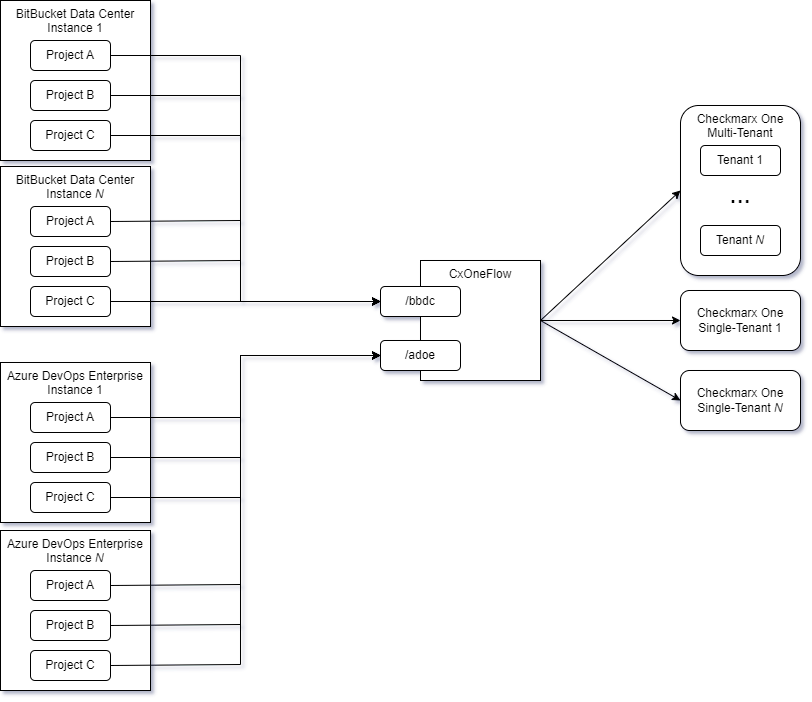
\includegraphics[width=\textwidth]{graphics/cxoneflow-deployment.png}
    \caption{\cxoneflow Deployment Diagram}
    \label{fig:cxoneflow-deployment}
\end{figure}

\section{Webhook Deployment Topology}

The goal of any \cxoneflow deployment is to enable webhook event delivery for a
large number of code repositories without a significant amount of effort.  Each 
SCM has several webhook deployment topologies that can be utilized to allow
deployment with the most minimal amount of effort. External factors can influence
what would be considered the most minimal amount of effort.

There are many factors that should be considered when considering the deployment
approach.  In some cases, some of the SCM webhook deployment capabilities may
not be utilized based on other considered factors.  Some of the
other factors to consider can include:

\begin{itemize}
    \item Administrative control of one or more SCM instances.
    \item Administrative control of multiple organizations in an SCM instance.
    \item Existing SCM integrations.
    \item Repository usage patterns that align with multiple development teams and Software Development Lifecycles.
\end{itemize}

This section is intended to provide a brief overview of the supported SCM repository organization topologies.
This overview is not comprehensive; a deeper look into your organization's SCMs may be required
to understand the full scope of deployment work. Part \ref{part:scms} of this manual covers the
details for integrating \cxoneflow with each supported SCM type.

The tool \extlink{https://github.com/checkmarx-ts/cxone-flow-audit}{cxone-flow-audit} has been
developed to assist in automating and auditing large scale deployments in some scenarios.  As
of the writing of this manual, the capabilities are limited to Azure DevOps.  As time progresses,
more deployment assistance capabilities will be added.


\subsection{BitBucket Data Center Webhook Topology}

\chapter{BitBucket Data Center}

\section{About BitBucket Data Center}

BitBucket Data Center is often confused with BitBucket Cloud; it should be noted that
the \cxoneflow configuration for BitBucket Data Center is not compatible with BitBucket Cloud.

\noindent\\The \cxoneflow endpoint \texttt{/bbdc} is the handler for all webhook event
payloads originating from BitBucket Data Center.  


\section{Webhook Configuration}

BitBucket Data Center can assign web hooks at the Project (aka Organization) level as well as at the
repository level.  Deploying web hook configurations for an enterprise-scale SCM is generally better
at the organization level since it will apply to all repositories in the organization.  Deploying
at the repository level is mostly suitable for testing purposes only.

Figure \ref{fig:bbdc-project-config} shows the BitBucket Data Center project configuration screen.  The
project key will appear in clone URLs and can be used as part of the regular expression 
placed in the \texttt{repo-match} configuration element.  Please see Section \ref{sec:scm-block-element} 
for a description of the \texttt{repo-match} configuration element.

The project's "Webhooks" configuration can be used to configure the \cxoneflow endpoint 
\texttt{/bbdc} to receive webhook events for each repository in the organization.  

\begin{figure}[h]
    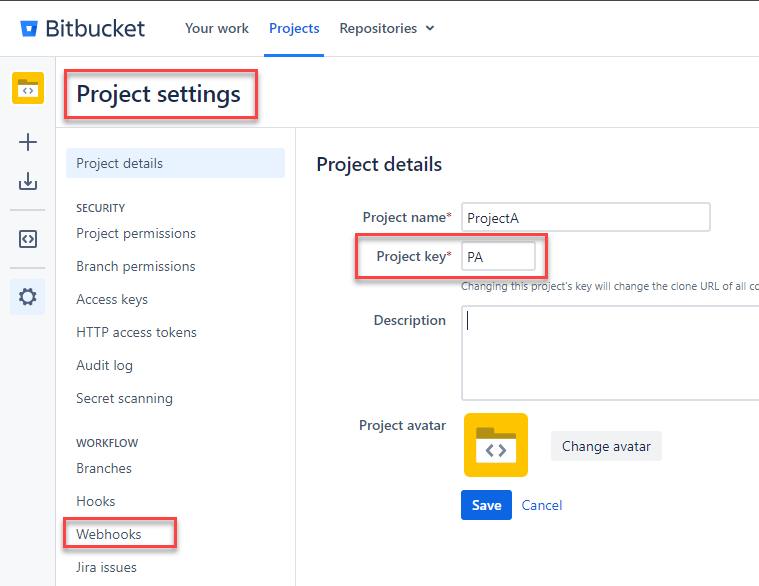
\includegraphics[width=\textwidth]{graphics/bbdc-project-config.png}
    \caption{BitBucket Data Center Project Configuration}
    \label{fig:bbdc-project-config}
\end{figure}

\begin{figure}[h]
    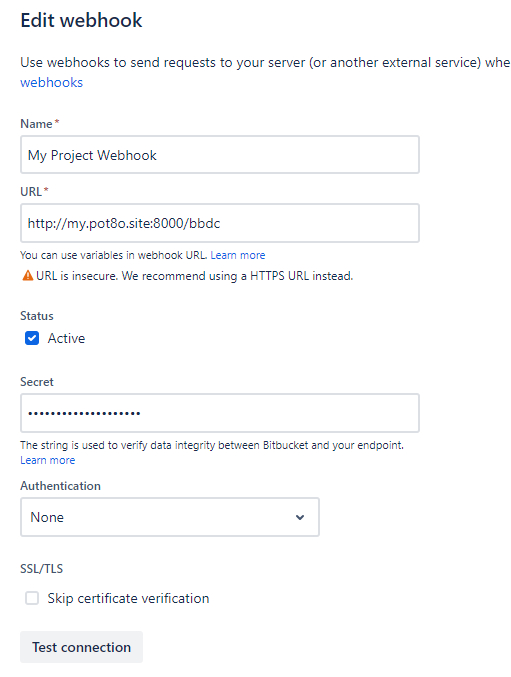
\includegraphics[width=\textwidth]{graphics/bbdc-webhook-config.png}
    \caption{BitBucket Data Center Webhook Configuration}
    \label{fig:bbdc-webhook-config}
\end{figure}



Figure \ref{fig:bbdc-webhook-config} shows a typical webhook configuration.  The Secret is how \cxoneflow
validates the origin of the event payload.  The configuration element \texttt{shared-secret}, as described
in Section \ref{sec:connection-element}, should be configured with the webhook secret value.  If \cxoneflow
is running at the specified URL endpoint, the "Test Connection" button will send a diagnostic ping
and receive back a positive response.  If the connection test fails, please ensure that \cxoneflow is running
at the address specified in the URL field and that the BitBucket Data Center server can make a connection
to that URL.

If the webhook is configured at the Project level, the events sent apply to all repositories contained
within the project.  Figure \ref{fig:bbdc-repo-event-config} shows the configured repository-level webhook 
events that will send a webhook payload to the \cxoneflow endpoint. 
Figure \ref{fig:bbdc-pr-event-config} shows the configured pull-request events that will be sent to 
the \cxoneflow endpoint.  The following events are currently supported:


\pagebreak
\begin{itemize}
    \item Repository Events
        \begin{itemize}
            \item Push
        \end{itemize}
    \item Pull Request Events
        \begin{itemize}
            \item Scanning Orchestration (Required)
                \begin{itemize}
                    \item Opened
                    \item Source branch updated
                    \item Modified
                \end{itemize}
        \end{itemize}
        \begin{itemize}
            \item Pull Request Scan Tagging (Optional)
                \begin{itemize}
                    \item Approved
                    \item Changes requested
                    \item Declined
                    \item Unapproved
                    \item Merged
                    \item Deleted
                \end{itemize}
        \end{itemize}

\end{itemize}


\begin{figure}[h]
    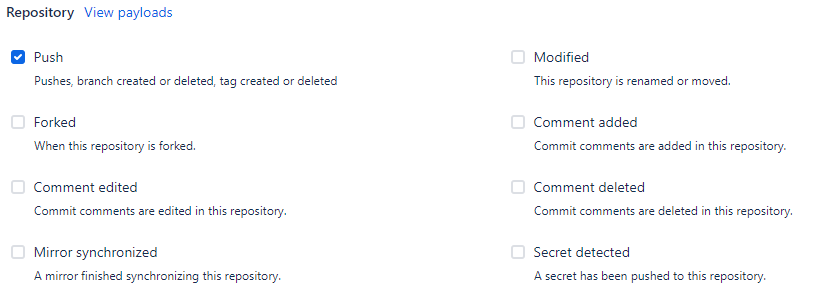
\includegraphics[width=\textwidth]{graphics/bbdc-repository-event-config.png}
    \caption{BitBucket Data Center Webhook Repository Event Config}
    \label{fig:bbdc-repo-event-config}
\end{figure}

\begin{figure}[h]
    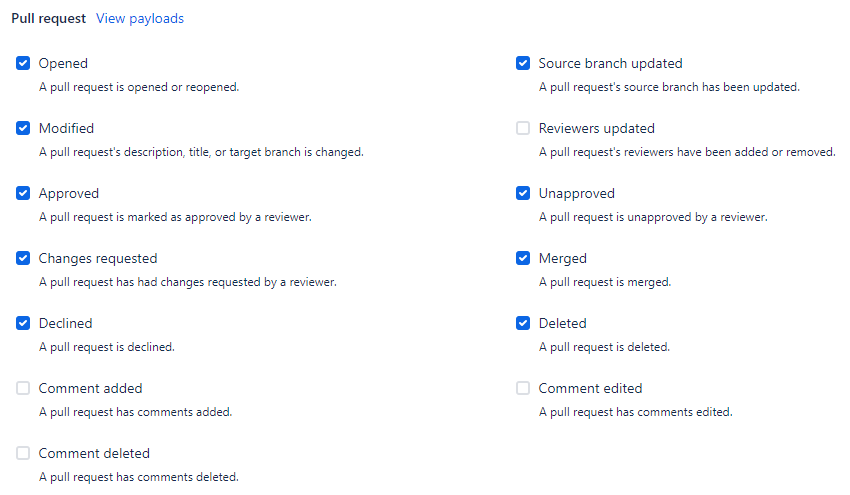
\includegraphics[width=\textwidth]{graphics/bbdc-pr-event-config.png}
    \caption{BitBucket Data Center Webhook Pull Request Event Config}
    \label{fig:bbdc-pr-event-config}
\end{figure}


\section{\cxoneflow HTTP Access Tokens}

While it is possible to use Basic Authorization to access the SCM, typically this is a configuration that
should be avoided.  The Basic Authorization is typically an interactive user account that can be subject
to password changes and Captcha verification that can break \cxoneflow operations.  It is generally
best to use a project-level HTTP Access Token for SCM connection configurations \texttt{api-auth} or
\texttt{clone-auth}.  Please refer to Section \ref{sec:connection-element} for more details about the token
configuration.

Figure \ref{fig:bbdc-token-config} shows the project-level "HTTP Access tokens" configuration.  The required
token permissions for \cxoneflow operations are:

\begin{itemize}
    \item Project read
    \item Repository read\footnote{Figure \ref{fig:bbdc-token-config} shows "Repository write".  There may be future versions of \cxoneflow that will need to create pull-request comments which will require write access.  If desired, the token can be granted "Repository read" until a write capability is released.}
\end{itemize}


\begin{figure}[h]
    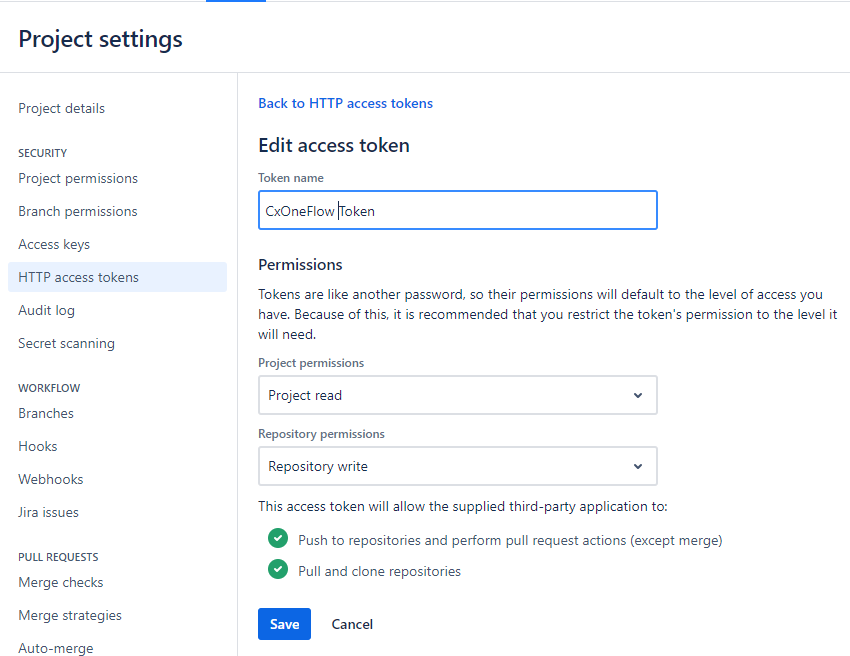
\includegraphics[width=\textwidth]{graphics/bbdc-token-config.png}
    \caption{BitBucket Data Center Project-Level HTTP Access Token Config}
    \label{fig:bbdc-token-config}
\end{figure}

Project-level access tokens do not have an associated user account.  If using project-level
access tokens, one project-level token is required per-project for which \cxoneflow is
orchestrating scans.

\section{\cxoneflow SSH Keys}

While performing scan orchestration, \cxoneflow does access the BitBucket Data Center API for
certain operations.  This requires a configuration in the \texttt{api-auth} configuration
element as described in Section \ref{sec:api-auth-element}.  The \texttt{clone-auth},
described in Section \ref{sec:clone-auth-element}, is an optional element where the credentials
used for cloning code can be provided.  If \texttt{clone-auth} is not provided, cloning will
be attempted using the credentials defined by \texttt{api-auth}.

The \texttt{clone-auth} configuration can define an SSH private key for use in cloning.  This
will allow for a separate set of credentials or authentication methods between cloning and
API use.


\section{Protected Branches}

The \cxoneflow workflow, as described in Section \ref{sec:overview}, uses the concept of "Protected Branches"
to know when to invoke workflows.  BitBucket Data Center allows for the configuration of the branching model
at the project and repository level.  Some repositories inherit their branching model from the project
configuration, but the ability for this to be overridden at the repository level is an optional configuration.
The branching model is used to determine which branches are "Protected Branches".

The project-level branching model configuration is shown in Figure \ref{fig:bbdc-branch-config}.  The
repository-level branching model configuration is similar in that both allow the definition of
"Development" and "Production" branches.  \cxoneflow considers any branch specified as a Development
or Production branch to be a "Protected Branch".

\begin{figure}[h]
    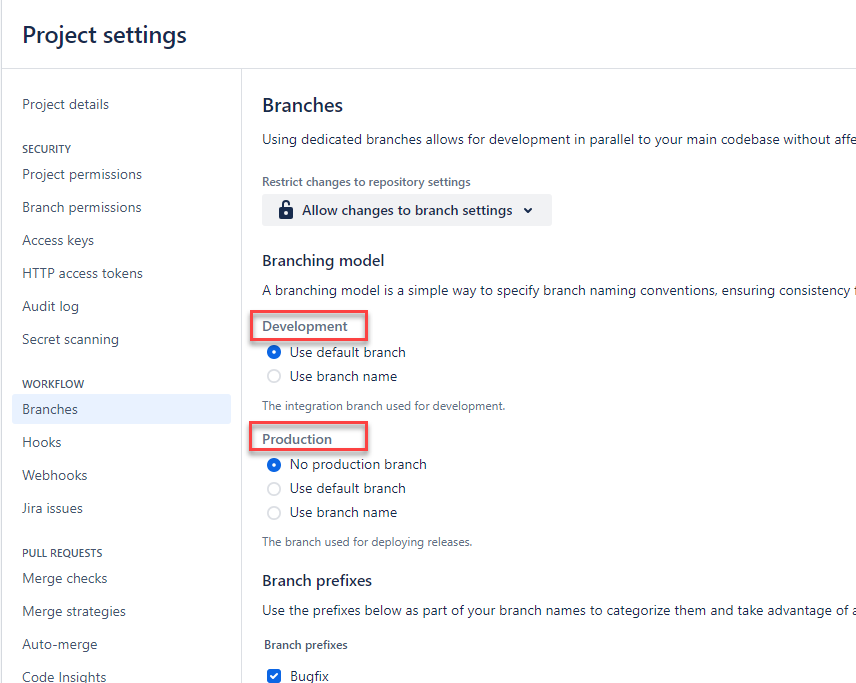
\includegraphics[width=\textwidth]{graphics/bbdc-branch-config.png}
    \caption{BitBucket Data Center Project-Level Branch Config}
    \label{fig:bbdc-branch-config}
\end{figure}



\subsection{Azure DevOps Webhook Topology}

Azure DevOps Enterprise (on-premise) uses one or more \textbf{Collection} logical units to separate
repositories into logical groups.  A \textbf{Collection} in Azure DevOps Enterprise 
corresponds to a Azure DevOps Cloud \textbf{Organization} in that the \textbf{Organization} is a logical unit 
that separates repositories into logical groups. Web hook deployments are not available at this scope.

In each \textbf{Collection} or \textbf{Organization}, zero or more \textbf{Project} logical
units establish the next level of repository organization.  Each \textbf{Project} will 
have one or more \textbf{Repository} units that will contain code that should be scanned.  Webhooks
can be deployed at this scope; each \textbf{Repository} in the configured \textbf{Project} logical unit
will emit webhook events when Service Hooks have been configured in the \textbf{Project} to
deliver webhook events to \cxoneflow.

Configuration of Service Hooks at the \textbf{Project} scope is generally the preferred
method of webhook deployment for Azure DevOps.

Webhooks can be deployed at the scope of each \textbf{Repository} if desired.  The number of repositories
in a large enterprise generally makes deployment at the \textbf{Repository} scope useful
only for testing purposes.


\subsection{GitHub Webhook Topology}

\chapter{GitHub Enterprise and GitHub Cloud}

\section{About GitHub}

The GitHub integration supports self-hosted GitHub Enterprise or GitHub Cloud.  The integration configurations
are virtually the same for each GitHub platform.  Minor differences may exist due to license or subscription
limitations of your GitHub platform type.  

The GitHub integration, as with other SCM integrations, uses web hooks to emit events to the \cxoneflow endpoint.
GitHub has both organization-level and repository-level webhook configurations
that can be used for simple integration scenarios.  \cxoneflow can also be configured as a GitHub Application
for easier deployment and visibility of deployment.

Deployment as a GitHub Application is the recommended deployment method.  It offers a single location where
\cxoneflow can be integrated into all organizations in a GitHub Enterprise instance or GitHub Cloud subscription.
When the GitHub application is defined by a logged in user, the scope of deployment may be limited by the access rights
the user has to each organization.  The \cxoneflow GitHub application runs with limited rights in each installed
organization, but it may require a user with administrative access across all organizations for deployment.


\section{GitHub Application Configuration}

\subsection{Configuring the Application Definition}

The GitHub Application definition determines the owner of the application.  The definition can
be created with an organization as owner or a user as owner.  The configuration method is the same
for each type of ownership.  Deploying with a user as application owner may be disruptive if the user
account is deleted or suspended.

\noindent\\Once the type of ownership is decided, the GitHub Application configuration page can be found in the following
locations:

\begin{itemize}
    \item \textbf{Organization Ownership:} Organization->Settings>Developer Settings->GitHub Apps
    \item \textbf{User Ownership:} User Icon (Top Right)->Settings->Developer Settings->GitHub Apps
\end{itemize}

\noindent\\The following steps can be followed to configure the \cxoneflow GitHub App:

\begin{enumerate}
    \item To start the configuration, click the button "New GitHub App". Figure \ref{fig:gh-new-app} shows
    the GitHub App page with the button to start the configuration in GitHub Enterprise.
    \item Provide a name for the GitHub App as depicted in Figure \ref{fig:gh-app-cfg-1}.  Any name
    can be used, but \cxoneflow is suggested.
    \item Optionally provide a description that is displayed to the users.
    \item Provide a URL that can be used to find information about the \cxoneflow GitHub App.  Any URL
    can be used; the URL to the \cxoneflow GitHub page \textbf{https://github.com/checkmarx-ts/cxone-flow}
    is suggested.
    \item Scroll to the \textbf{Webhook} configuration section; the settings prior to the web hook configuration
    are optional and not used by \cxoneflow.
    \item Provide the URL to the \cxoneflow endpoint with the \textbf{/gh} suffix as shown in Figure \ref{fig:gh-app-cfg-2}.
    \item Provide the web hook secret value that is configured in the \cxoneflow YAML as described in Section \ref{sec:yaml-config}.
    \item Scroll the the \textbf{Permissions} section and expand the \textbf{Repository Permissions} as shown in
    Figure \ref{fig:gh-app-cfg-3}.  The following permissions are required:
    \begin{itemize}
        \item Contents: Read-only
        \item Pull requests: Read and write
    \end{itemize}
    \item Scroll to the \textbf{Subscribe to events} section as shown in Figure \ref{fig:gh-app-cfg-4}.  The following events are required:
    \begin{itemize}
        \item Pull request
        \item Pull request review
        \item Push
    \end{itemize}
    \item Scroll to the \textbf{Where can this GitHub App be installed?} section and select \textbf{Any account} as shown in
    Figure \ref{fig:gh-app-cfg-5}.
    \item Click the \textbf{Create GitHub App} button.
    \item After the application is created, open the application settings \textbf{General} tab and scroll to the
    \textbf{Private keys} section as shown in Figure \ref{fig:gh-app-cfg-6}.
    \item Click the \textbf{Generate a private key} button.  A private key entry will appear and a file download will start.
    The contents of the download file is the PEM encoded private key that is to be stored as a secret.  See Section
    \ref{sec:yaml-config} for configuration instructions to reference this GitHub App private key.
\end{enumerate}

\begin{figure}[ht]
    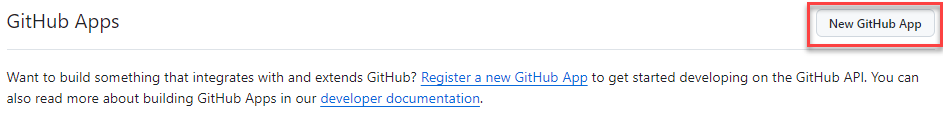
\includegraphics[width=\textwidth]{graphics/gh-new-app.png}
    \caption{New GitHub App Button}
    \label{fig:gh-new-app}
\end{figure}


\begin{figure}[ht]
    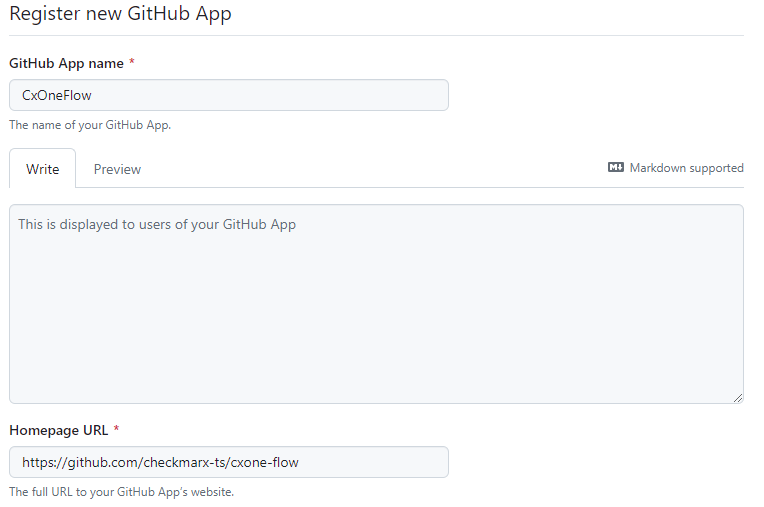
\includegraphics[width=\textwidth]{graphics/gh-app-cfg-1.png}
    \caption{GitHub App Name and URL Configuration}
    \label{fig:gh-app-cfg-1}
\end{figure}

\begin{figure}[ht]
    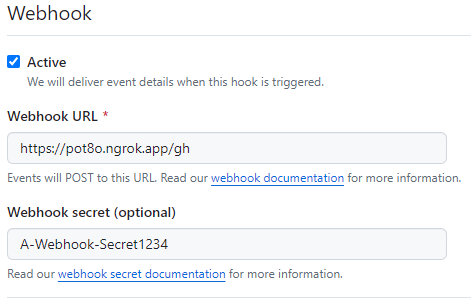
\includegraphics[width=\textwidth]{graphics/gh-app-cfg-2.png}
    \caption{GitHub App Webhook Configuration}
    \label{fig:gh-app-cfg-2}
\end{figure}

\begin{figure}[ht]
    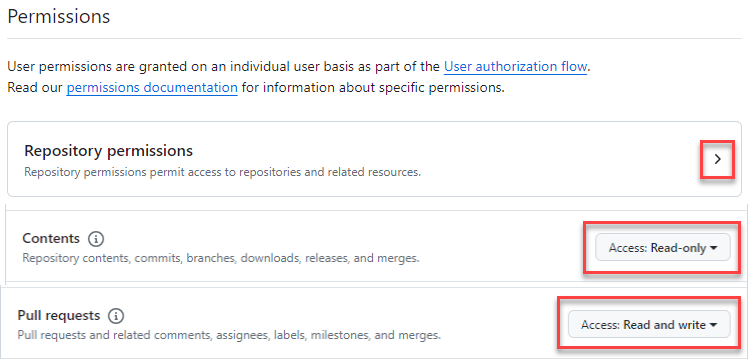
\includegraphics[width=\textwidth]{graphics/gh-app-cfg-3.png}
    \caption{GitHub App Permissions}
    \label{fig:gh-app-cfg-3}
\end{figure}

\begin{figure}[ht]
    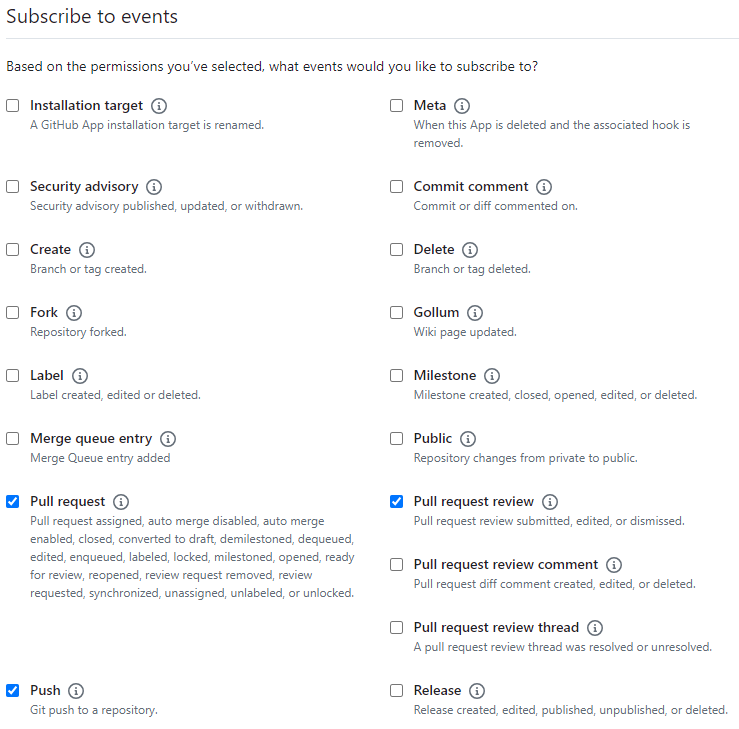
\includegraphics[width=\textwidth]{graphics/gh-app-cfg-4.png}
    \caption{GitHub App Event Subscriptions}
    \label{fig:gh-app-cfg-4}
\end{figure}

\begin{figure}[ht]
    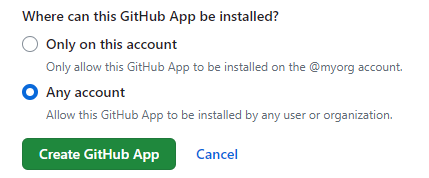
\includegraphics[width=\textwidth]{graphics/gh-app-cfg-5.png}
    \caption{GitHub App Install Scope}
    \label{fig:gh-app-cfg-5}
\end{figure}

\begin{figure}[ht]
    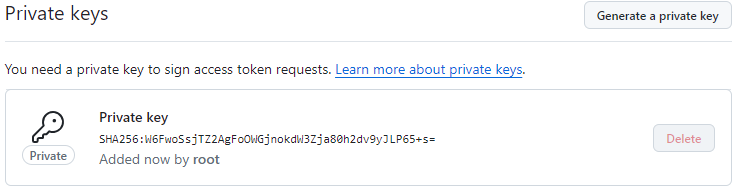
\includegraphics[width=\textwidth]{graphics/gh-app-cfg-6.png}
    \caption{GitHub App Private Keys}
    \label{fig:gh-app-cfg-6}
\end{figure}

\FloatBarrier

\subsection{Deploying the Application}

\textbf{Before deploying the application, it is recommended to configure the \cxoneflow YAML
so the endpoint will recognize events sent by the application.  See Section \ref{sec:gh-yaml-config} for guidance on the \cxoneflow
GitHub configuration.}

\noindent\\After the application is defined, deployment is performed from the application
definition page. The following steps can be followed to deploy the \cxoneflow GitHub App:

\begin{enumerate}
    \item Navigate to the GitHub App definition page and click the \textbf{Edit} button for the \cxoneflow
    application definition.  An example of this view is shown in Figure \ref{fig:gh-app-deploy-1}.
    \item Select the \textbf{Install App} tab on the left side of the view.  Figure \ref{fig:gh-app-deploy-2}
    shows the install view.\footnote{If the view shows only the organization that owns the \cxoneflow GitHub App definition,
    then the application visibility is configured to be private.  The application must be public to install in other organizations.}
    \item Click the \textbf{Install} button next to the organization where the application should be installed.
    \item An installation confirmation similar to that shown in Figure \ref{fig:gh-app-deploy-3} will be displayed.
    Click the \textbf{Install} button to complete installation.
    \item Repeat these steps to install the \cxoneflow GitHub App in all desired organizations.  Figure \ref{fig:gh-app-deploy-4}
    shows the view where the GitHub App has been installed in multiple organizations.
\end{enumerate}

\begin{figure}[ht]
    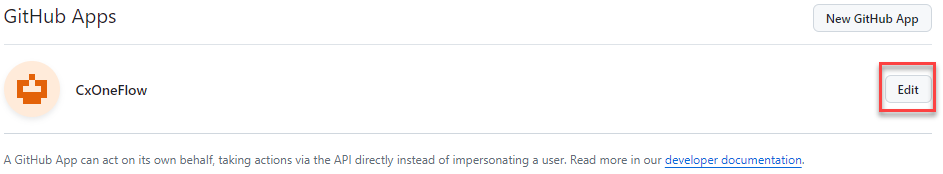
\includegraphics[width=\textwidth]{graphics/gh-app-deploy-1.png}
    \caption{GitHub App List}
    \label{fig:gh-app-deploy-1}
\end{figure}

\begin{figure}[ht]
    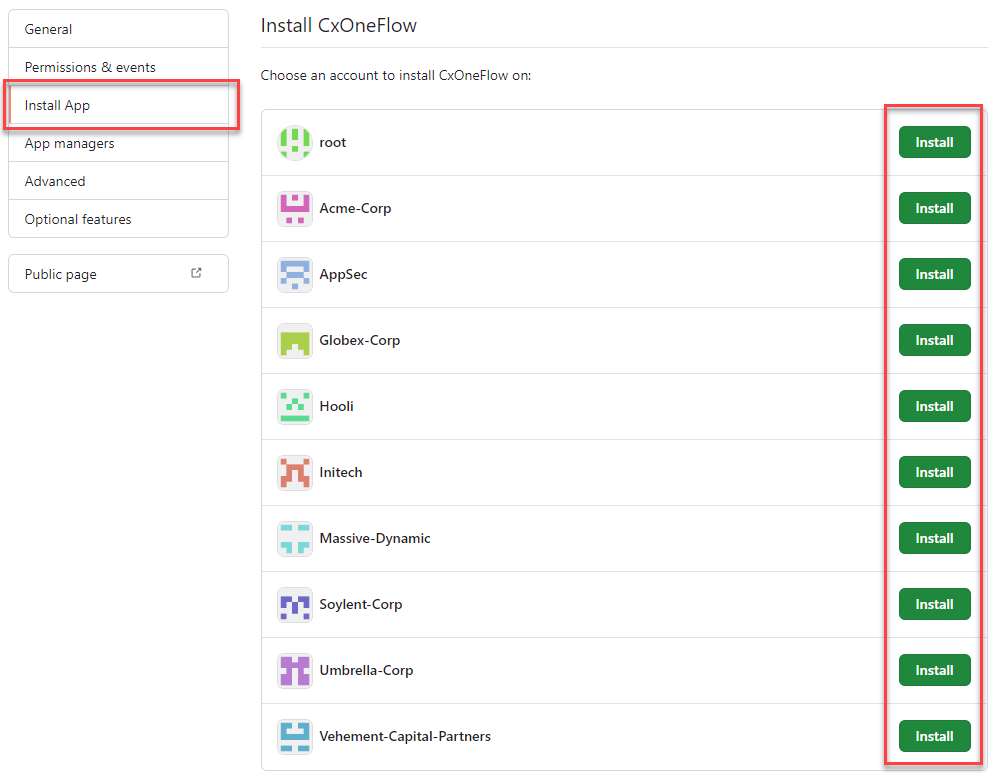
\includegraphics[width=\textwidth]{graphics/gh-app-deploy-2.png}
    \caption{GitHub App Install View}
    \label{fig:gh-app-deploy-2}
\end{figure}

\begin{figure}[ht]
    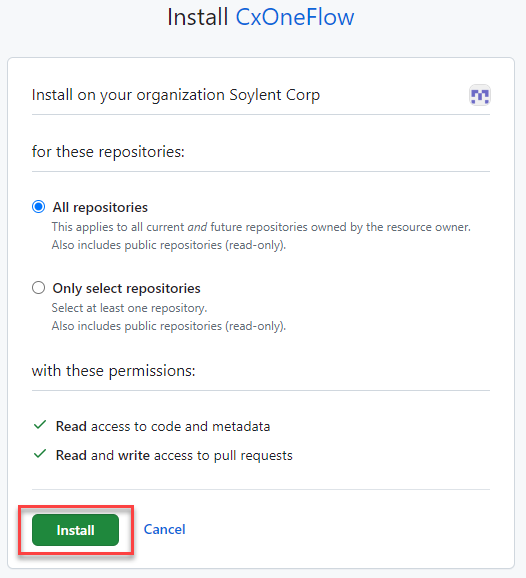
\includegraphics[width=\textwidth]{graphics/gh-app-deploy-3.png}
    \caption{GitHub App Install Confirmation}
    \label{fig:gh-app-deploy-3}
\end{figure}

\begin{figure}[ht]
    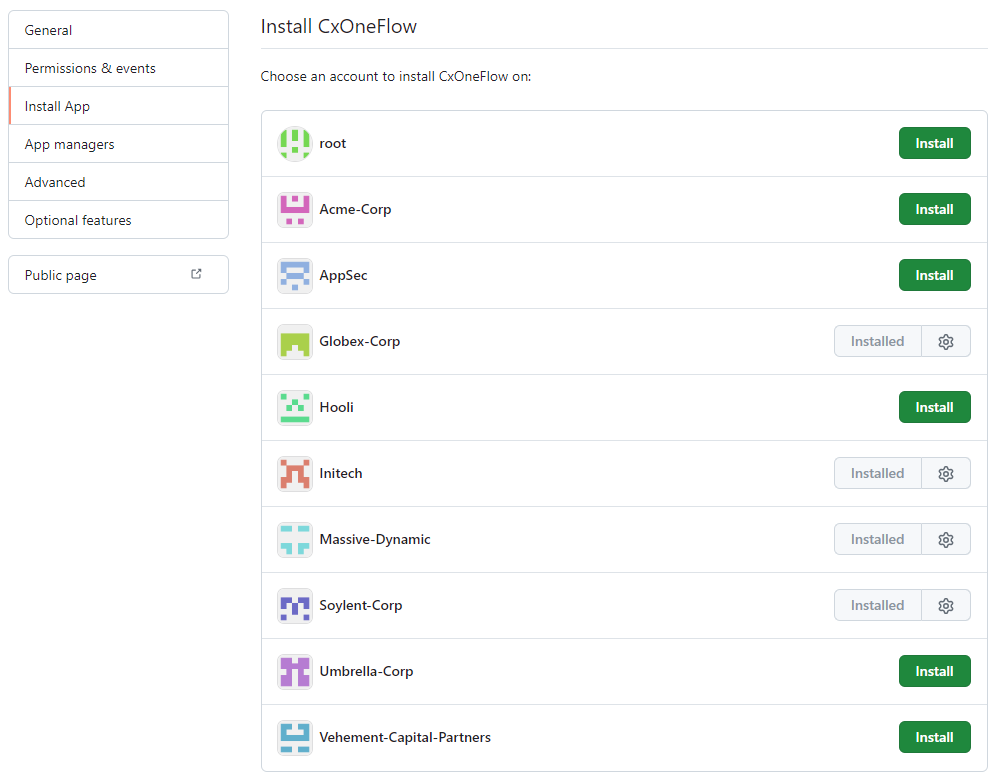
\includegraphics[width=\textwidth]{graphics/gh-app-deploy-4.png}
    \caption{GitHub App Installed Organization View}
    \label{fig:gh-app-deploy-4}
\end{figure}

\FloatBarrier

\subsection{GitHub App Management Recommendations}

\subsubsection{Repository Scope}

It is recommended that the application is installed for all repositories in an organization.  While it is possible to limit the
application to specific repositories, modifications to change the selected repositories may be difficult to manage.  Limiting
the repository scope may be useful for testing purposes but impractical for normal operations.

\subsubsection{Organization User App Management Permissions}

In each organization, a number of users may have the rights to manage applications that are installed on that organization.  It is
recommended to restrict the ability of organization users to manage installed applications.  Each organization user that can manage
GitHub Apps in that organization can suspend or remove the \cxoneflow application installation.

If the \cxoneflow application is deleted, this will be reflected in the \textbf{Install App} view as shown in Figure \ref{fig:gh-app-deploy-4}.
This is easy to periodically audit and discover when the application has been removed from an organization unintentionally or otherwise.
If the application is simply suspended, the \textbf{Install App} view will indicate the application is installed but will not indicate
that operation has been suspended.

The \cxoneflow logs do emit log entries when the GitHub App is suspended or removed. The listing below shows example log events
emitted when a user has modified the GitHub App on an organization.  If desired, monitoring for these log events may provide
an automated method of auditing when the GitHub App is no longer active for an organization.

\begin{code}{GitHub App Example Events}{}{}
[2024-10-03T13:10:30+0000][3219][GithubOrchestrator][INFO] Install event 'suspend': Initiated by [root] on Organization [Initech]
[2024-10-03T13:11:02+0000][3219][GithubOrchestrator][INFO] Install event 'deleted': Initiated by [root] on Organization [Initech]
\end{code}

\section{Webhook Configuration}

If it is not possible to use the GitHub App for \cxoneflow integration, webhook definitions can be configured at either the
organization or repository level.  When using webhooks instead of a GitHub App, please be aware of the following:

\begin{itemize}
    \item A user token (PAT) with appropriate permissions to all repositories in the scope of install must be used for API access.
    \item If cloning must be performed with an SSH key, the user that owns the SSH key must also have appropriate permissions for
    all repositories in scope.
    \item The webhook integration settings must be performed multiple times:
    \begin{itemize}
        \item Configuring it at the organization level will apply for all repositories in the organization; the configuration must be repeated for
        every organization.
        \item Configuring at the repository level will apply only for that repository; the configuration must be repeated for every
        repository.
    \end{itemize}
\end{itemize}

\noindent\\The webhook configuration in GitHub Enterprise and GitHub Cloud is the same.  They are referred to as \textbf{Hooks} in
GitHub Enterprise and \textbf{Webhooks} in GitHub Cloud.  Webhook integration can be performed with the following steps:

\begin{enumerate}
    \item Locate the webhook configuration page at the organization or repository scope as appropriate for your
    GitHub platform.
    \item Click the \textbf{Add webhook} button.
    \item Refer to Figure \ref{fig:gh-webhook-1} to configure the webhook payload delivery options:
    \begin{enumerate}
        \item Configure the payload URL with the \cxoneflow endpoint url with the \textbf{/gh} path suffix.
        \item Set the content type to \textbf{application/json}.
        \item Supply the webhook secret that is configured as the \texttt{shared-secret} as described in
        Section \ref{sec:yaml-config}.
    \end{enumerate}
    \item In the section \textbf{Which events would you like to trigger this webhook?}, the option \textbf{Send me everything}
    will work but is not recommended as the \cxoneflow endpoint will receive many events it will not handle.  Using the
    \textbf{Let me select individual events} option with the following events is recommended:
    \begin{itemize}
        \item Pushes
        \item Pull requests
        \item Pull request reviews
    \end{itemize}
    \item Click the \textbf{Add webhook} button to complete the webhook configuration.
\end{enumerate}

\begin{figure}[ht]
    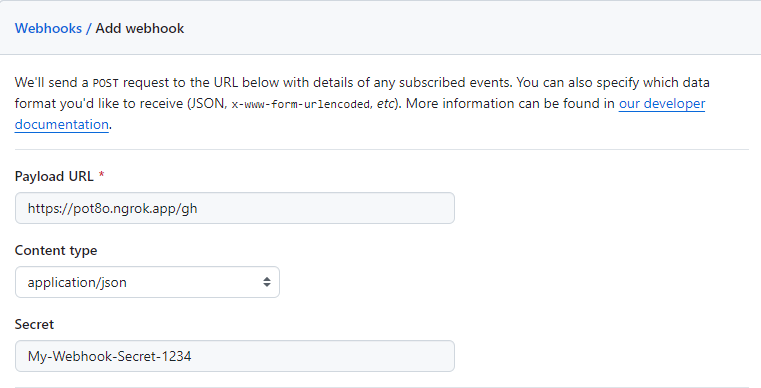
\includegraphics[width=\textwidth]{graphics/gh-webhook-1.png}
    \caption{GitHub Webhook Payload Configuration}
    \label{fig:gh-webhook-1}
\end{figure}



\FloatBarrier

\section{\cxoneflow YAML Configuration}\label{sec:gh-yaml-config}

This section is intended to show some of the GitHub-specific requirements for successful configuration.  The differences
between GitHub Enterprise and GitHub Cloud are minimal; generally the differences are related to how API and display URLs
work.

\subsection{GitHub Enterprise}

Below is a listing of a minimal GitHub Enterprise YAML configuration.  The elements to note in this
configuration:

\begin{itemize}
    \item The \texttt{base-url} is the root URL for the GitHub Enterprise instance.  This URL is also used
    when forming display links such as links to code in PR comments.
    \item The \texttt{api-url-suffix} is the path extension appended to \texttt{base-url} for API requests.
    \item Since this service definition is for a GitHub App, the \texttt{app-private-key} points to the secret
    containing the generated private key.
    \item Since the GitHub App permissions should be allowed to read repository contents, there is no need
    to provide a \texttt{clone-auth} configuration.
\end{itemize}

\begin{code}{Minimal YAML Configuration Example}{GitHub Enterprise as GitHub App}{}
secret-root-path: /run/secrets
server-base-url: https://cxoneflow.mydomain.com:8443/

gh:
    - service-name: GHE
      repo-match: .*
      feedback:
        pull-request:
          enabled: True
      connection:
        base-url: https://scm.corp.com
        api-url-suffix: api/v3
        shared-secret: scm-shared-secret
        api-auth:
          app-private-key: ghe-app-priv-key
      cxone:
        tenant: mytenant
        oauth:
          client-id: my-oauth-id
          client-secret: my-oauth-secret
        iam-endpoint: US
        api-endpoint: US
\end{code}


\subsection{GitHub Cloud}

Below is a listing of a minimal GitHub Cloud YAML configuration.  The elements to note in this
configuration:

\begin{itemize}
    \item The \texttt{base-url} is the root URL for the GitHub Cloud API.
    \item The \texttt{base-display-url} is the root URL for the GitHub Cloud UI. This URL is used
    when forming display links such as links to code in PR comments since the API URL does not
    provide interactive content.
    \item There is no \texttt{api-url-suffix} since the \texttt{base-url} is the root for API requests.
    \item Since this service definition is for a GitHub App, the \texttt{app-private-key} points to the secret
    containing the generated private key.
    \item Since the GitHub App permissions should be allowed to read repository contents, there is no need
    to provide a \texttt{clone-auth} configuration.
\end{itemize}

\begin{code}{Minimal YAML Configuration Example}{GitHub Cloud as GitHub App}{}
secret-root-path: /run/secrets
server-base-url: https://cxoneflow.mydomain.com:8443/

gh:
    - service-name: GHC
      repo-match: .*
      feedback:
        pull-request:
          enabled: True
      connection:
        base-url: https://api.github.com
        base-display-url: https://www.github.com
        shared-secret: scm-shared-secret
        api-auth:
          app-private-key: ghc-app-priv-key
      cxone:
        tenant: mytenant
        oauth:
          client-id: my-oauth-id
          client-secret: my-oauth-secret
        iam-endpoint: US
        api-endpoint: US
\end{code}
  

\section{Protected Branches}

GitHub allows a default branch to be defined for each repository.  A default branch name is defined at the organization
level and is initially inherited by each repository in the organization.  The default branch may be changed in the repository
to any branch defined in the repository. If there are no branch protection rules for the repository generating a webhook event, 
the default branch for the repository is assumed to be a protected branch.

Branch protection rules can be defined at both the organization and repository levels.  If there are any branches
defined as protected via the branch protection rules, those branches are considered protected branches.  When branch protection
rules define protected branches, the repository default branch is not considered as a protected branch unless it is also included
as a protected branch in the branch protection rules.


\subsection{Gitlab Webhook Topology}

\chapter{Self-Hosted Gitlab and Gitlab Cloud}


\section{About Gitlab}

The Gitlab integration supports both self-hosted and cloud-hosted Gitlab instances.  Each type
of Gitlab instance uses a subscription model that can limit access to some of the webhook
deployment features that can be utilized by \cxoneflowns. The effort to deploy \cxoneflow at scale
across a large number of repositories can change based upon the level of subscription
and how the Gitlab instance is hosted.

The \cxoneflow endpoint \texttt{/gl} is the handler for all webhook event
payloads originating from any Gitlab instance type.  


\section{Webhook Topology}

\chapter{Self-Hosted Gitlab and Gitlab Cloud}


\section{About Gitlab}

The Gitlab integration supports both self-hosted and cloud-hosted Gitlab instances.  Each type
of Gitlab instance uses a subscription model that can limit access to some of the webhook
deployment features that can be utilized by \cxoneflowns. The effort to deploy \cxoneflow at scale
across a large number of repositories can change based upon the level of subscription
and how the Gitlab instance is hosted.

The \cxoneflow endpoint \texttt{/gl} is the handler for all webhook event
payloads originating from any Gitlab instance type.  


\section{Webhook Topology}

\chapter{Self-Hosted Gitlab and Gitlab Cloud}


\section{About Gitlab}

The Gitlab integration supports both self-hosted and cloud-hosted Gitlab instances.  Each type
of Gitlab instance uses a subscription model that can limit access to some of the webhook
deployment features that can be utilized by \cxoneflowns. The effort to deploy \cxoneflow at scale
across a large number of repositories can change based upon the level of subscription
and how the Gitlab instance is hosted.

The \cxoneflow endpoint \texttt{/gl} is the handler for all webhook event
payloads originating from any Gitlab instance type.  


\section{Webhook Topology}

\input{scms/topology/gl.tex}


\section{\cxoneflowtext\space YAML Configuration for GitLab}

Below is a listing of a minimal Gitlab YAML configuration.  The elements to note in this
configuration:

\begin{itemize}
    \item The \texttt{base-url} is the root URL for the Gitlab instance.  This URL is also used
    when forming display links such as links to code in PR comments.
    \item The \texttt{api-url-suffix} is the path extension appended to \texttt{base-url} for API requests.
    \item The \texttt{repo-match} regular expression matches the service definition with events emitted by any repository
    in the Gitlab instance.
\end{itemize}

\input{operation/gl_minimal_example.tex}

\section{Deploying Webhook Configurations in Gitlab}

The scope where webhooks are deployed for \cxoneflow will determine how to provision a PAT
that has the appropriate permissions to the projects in the deployment scope.  Using service
hooks, for example, requires a PAT from a user that has access to all projects in the Gitlab
instance.

Deploying webhooks at the project or group scope requires a PAT from a user that has access
to the projects in the deployed scope.  This may require multiple \cxoneflow service definitions
with the \texttt{repo-match} regular expression such that events in the scope available to a
PAT are handled properly.

A PAT, regardless of user or scope, requires the following permissions:

\begin{itemize}
  \item api
  \item api\_read
  \item ai features
\end{itemize}

\subsection{Service Hooks}

A Gitlab administrator can configure system-wide service hooks.  The service hooks configuration is located in the
administrative configuration menu, accessible by clicking the "Admin" button as shown in Figure \ref{fig:gl-admin-menu}.

\begin{figure}[ht]
  \centering
  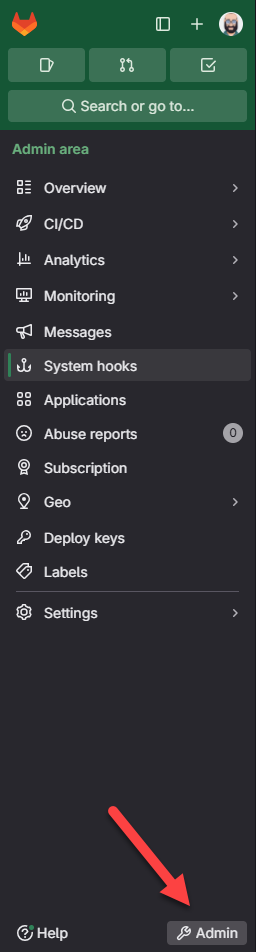
\includegraphics[scale=.5]{graphics/gl-system-hook-admin.png}
  \caption{Gitlab System Hook Administration Menu}
  \label{fig:gl-admin-menu}
\end{figure}


An example service hook definition is shown in Figure \ref{fig:gl-service-hook-def}.  The following are
required configuration elements:

\begin{itemize}
  \item The URL to the \cxoneflow instance ending with the \texttt{gl} route.
  \item The value provided in the \texttt{shared-secret} element under the \texttt{connection} element in the service definition.
  \item The triggers should be \textbf{Push events} and \textbf{Merge request events}.
\end{itemize}

Click the "Add webhook" button to deploy the service hook definition.  Gitlab will immediately start delivering
events to the configured \cxoneflow endpoint.

\begin{figure}[ht]
  \centering
  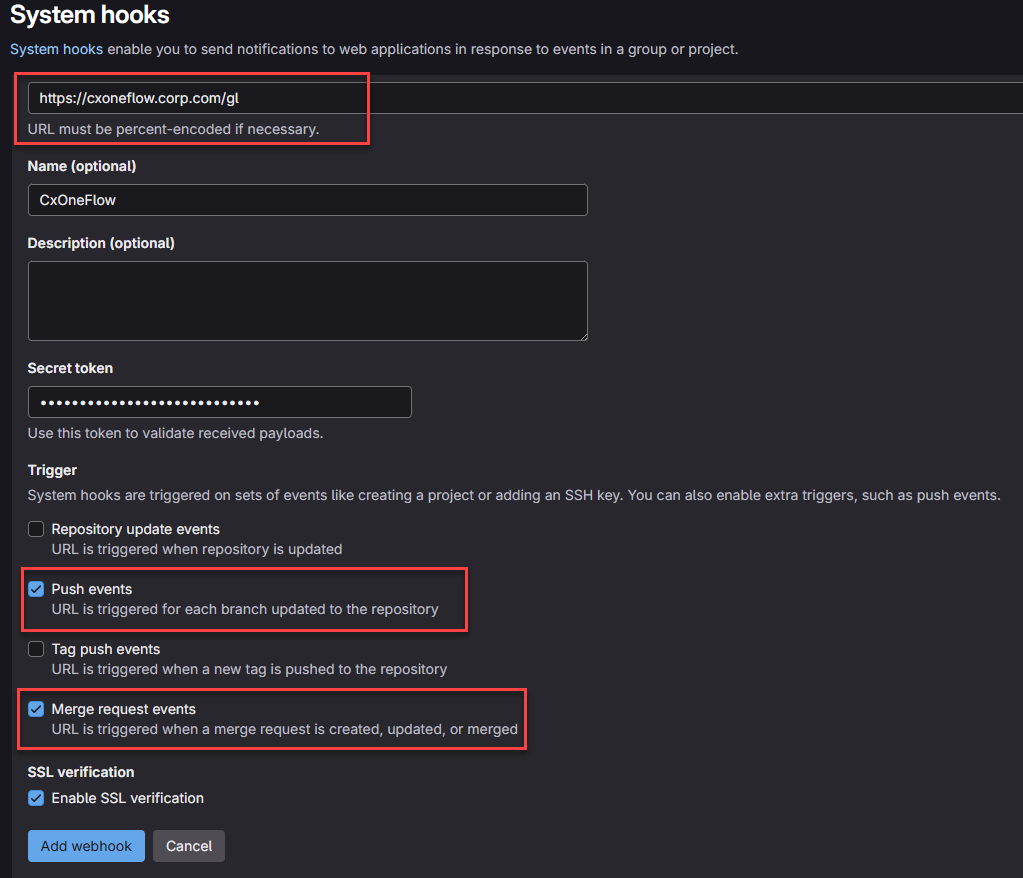
\includegraphics[width=\textwidth]{graphics/gl-service-hooks.png}
  \caption{Gitlab System Hook Definition}
  \label{fig:gl-service-hook-def}
\end{figure}

\subsection{Group or Project Webhooks}

Webhook configurations at the group or project scope operate the same.  The settings for each
are accessed by navigating to the group or project view and selecting \textbf{Settings->Webhooks}.
If attempting to configure webhooks at the group scope in a free Gitlab self-hosted instance or
a free Gitlab cloud account, you will be prompted to purchase a license.

The webhook configuration can be initiated by clicking the \textbf{Add new webhook} button. Figure \ref{fig:gl-project-1}
shows the endpoint configuration where the URL for the \cxoneflow instance with the \texttt{gl} is provided
along with the shared secret.  The shared secret value should match the value provided in the
\texttt{shared-secret} element under the \texttt{connection} element in the service definition.

\begin{figure}[ht]
  \centering
  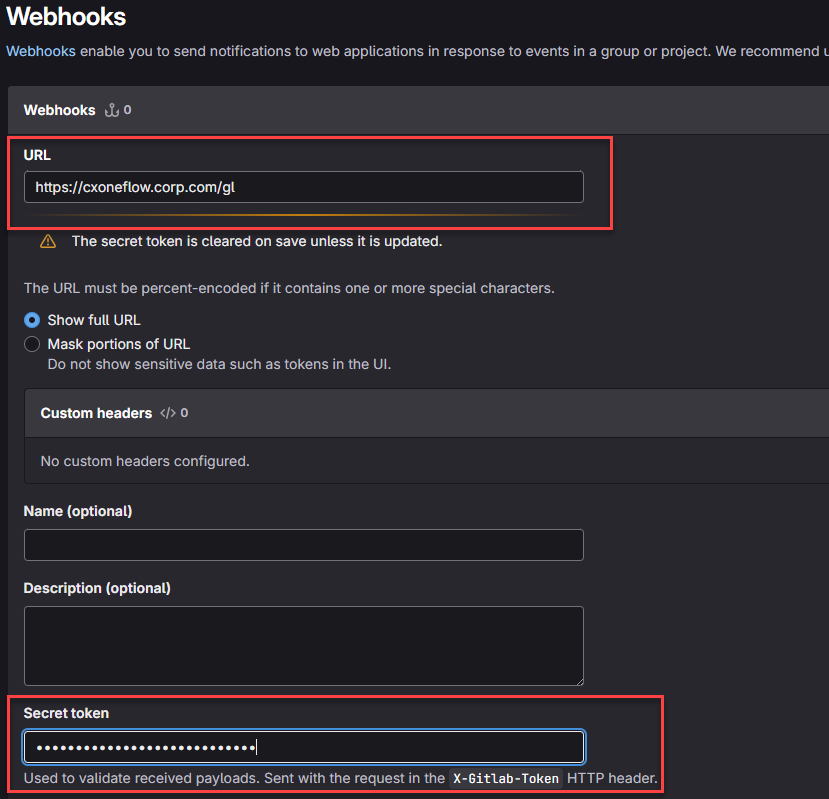
\includegraphics[width=\textwidth]{graphics/gl-project-hook-1.png}
  \caption{Gitlab Group/Project Webhook Endpoint Configuration}
  \label{fig:gl-project-1}
\end{figure}

Figure \ref{fig:gl-project-2} shows the webhook configured to send events for 
\textbf{Push events} and \textbf{Merge request events}.  While it is possible to filter
which branches emit push events, doing so may cause \cxoneflow to not work as expected.

Click the "Add webhook" button to deploy the webhook definition.  Gitlab will immediately start delivering
events to the configured \cxoneflow endpoint.


\begin{figure}[ht]
  \centering
  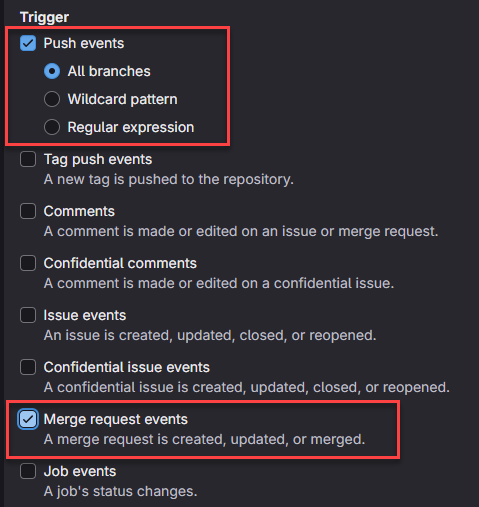
\includegraphics[width=\textwidth]{graphics/gl-project-hook-2.png}
  \caption{Gitlab Group/Project Webhook Event Configuration}
  \label{fig:gl-project-2}
\end{figure}



\section{Protected Branches}

Gitlab allows for a group scope definition of a "default branch" that can be overridden at the
project scope.  The default branch may be considered a protected branch (e.g. it limits who can
commit to the default branch), but Gitlab does not require the default branch to be a protected
branch.  For consistency with \cxoneflow workflow logic with other SCMs, the default branch is
considered a protected branch for all event handling workflows.  This means a push to the 
default branch or a merge request targeting the default branch will initiate a scan regardless
of the configured protection status.

Branch protection rules other than those associated with the default branch can be configured at
the project scope.  The rules allow a named branch to be configured as protected or to supply
a wildcard to protect branches with names that match the wildcard specification.  \cxoneflow will
follow the Gitlab configuration logic for protected branches when handling an event.  Any push
or merge request targeting a protected branch will initiate a scan.



\section{\cxoneflowtext\space YAML Configuration for GitLab}

Below is a listing of a minimal Gitlab YAML configuration.  The elements to note in this
configuration:

\begin{itemize}
    \item The \texttt{base-url} is the root URL for the Gitlab instance.  This URL is also used
    when forming display links such as links to code in PR comments.
    \item The \texttt{api-url-suffix} is the path extension appended to \texttt{base-url} for API requests.
    \item The \texttt{repo-match} regular expression matches the service definition with events emitted by any repository
    in the Gitlab instance.
\end{itemize}

\begin{code}{Minimal YAML Configuration Example}{Gitlab Webhooks}{}
  secret-root-path: /run/secrets
  server-base-url: https://cxoneflow.mydomain.com:8443/
  
  gh:
      - service-name: Gitlab
        repo-match: ^http(s)?:(\/){2}gitlab\.corp\.com.*
        feedback:
          pull-request:
            enabled: True
        connection:
          base-url: https://gitlab.corp.com
          api-url-suffix: api/v4
          shared-secret: scm-shared-secret
          api-auth:
            token: ghe-token
        cxone:
          tenant: mytenant
          oauth:
            client-id: my-oauth-id
            client-secret: my-oauth-secret
          iam-endpoint: US
          api-endpoint: US
\end{code}
    

\section{Deploying Webhook Configurations in Gitlab}

The scope where webhooks are deployed for \cxoneflow will determine how to provision a PAT
that has the appropriate permissions to the projects in the deployment scope.  Using service
hooks, for example, requires a PAT from a user that has access to all projects in the Gitlab
instance.

Deploying webhooks at the project or group scope requires a PAT from a user that has access
to the projects in the deployed scope.  This may require multiple \cxoneflow service definitions
with the \texttt{repo-match} regular expression such that events in the scope available to a
PAT are handled properly.

A PAT, regardless of user or scope, requires the following permissions:

\begin{itemize}
  \item api
  \item api\_read
  \item ai features
\end{itemize}

\subsection{Service Hooks}

A Gitlab administrator can configure system-wide service hooks.  The service hooks configuration is located in the
administrative configuration menu, accessible by clicking the "Admin" button as shown in Figure \ref{fig:gl-admin-menu}.

\begin{figure}[ht]
  \centering
  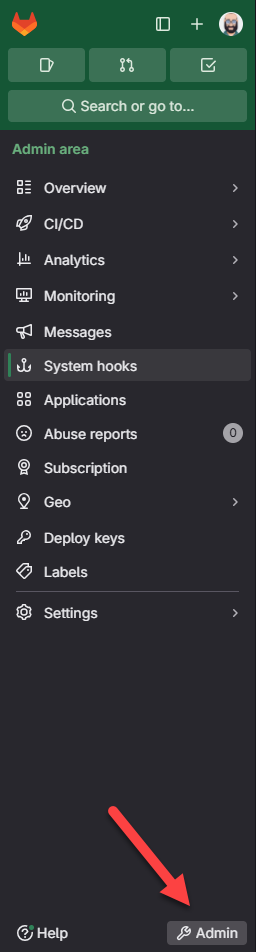
\includegraphics[scale=.5]{graphics/gl-system-hook-admin.png}
  \caption{Gitlab System Hook Administration Menu}
  \label{fig:gl-admin-menu}
\end{figure}


An example service hook definition is shown in Figure \ref{fig:gl-service-hook-def}.  The following are
required configuration elements:

\begin{itemize}
  \item The URL to the \cxoneflow instance ending with the \texttt{gl} route.
  \item The value provided in the \texttt{shared-secret} element under the \texttt{connection} element in the service definition.
  \item The triggers should be \textbf{Push events} and \textbf{Merge request events}.
\end{itemize}

Click the "Add webhook" button to deploy the service hook definition.  Gitlab will immediately start delivering
events to the configured \cxoneflow endpoint.

\begin{figure}[ht]
  \centering
  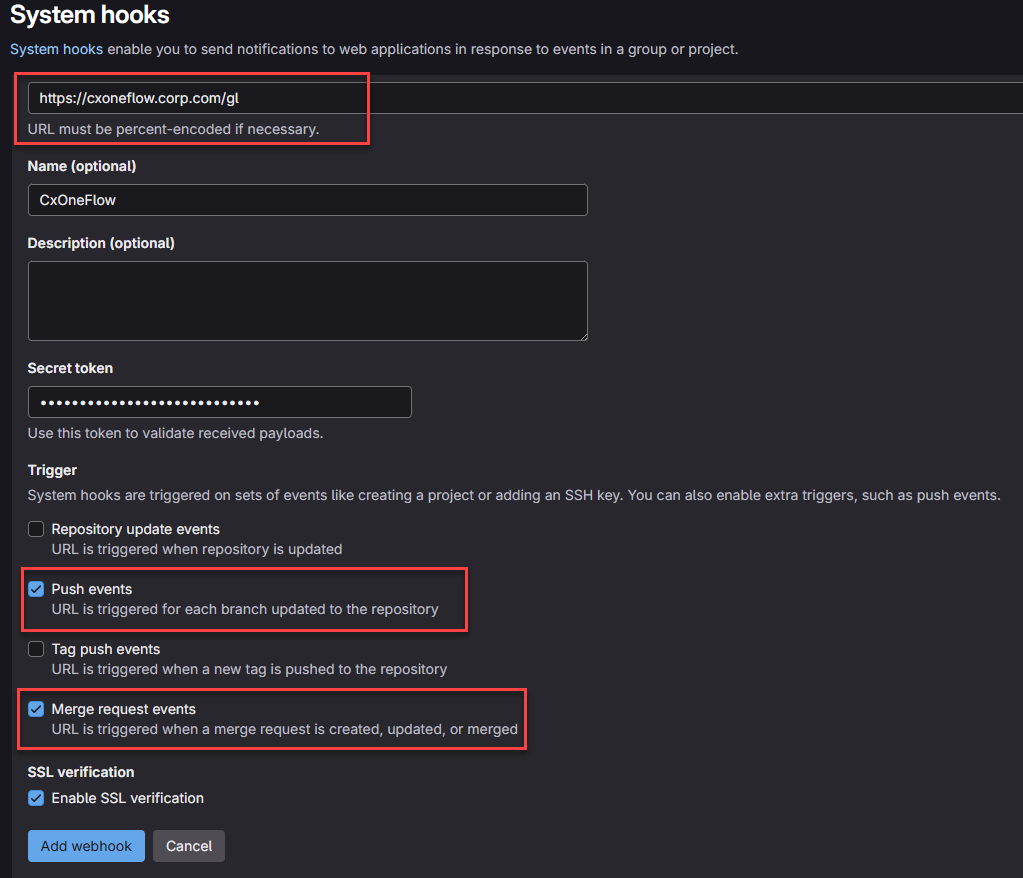
\includegraphics[width=\textwidth]{graphics/gl-service-hooks.png}
  \caption{Gitlab System Hook Definition}
  \label{fig:gl-service-hook-def}
\end{figure}

\subsection{Group or Project Webhooks}

Webhook configurations at the group or project scope operate the same.  The settings for each
are accessed by navigating to the group or project view and selecting \textbf{Settings->Webhooks}.
If attempting to configure webhooks at the group scope in a free Gitlab self-hosted instance or
a free Gitlab cloud account, you will be prompted to purchase a license.

The webhook configuration can be initiated by clicking the \textbf{Add new webhook} button. Figure \ref{fig:gl-project-1}
shows the endpoint configuration where the URL for the \cxoneflow instance with the \texttt{gl} is provided
along with the shared secret.  The shared secret value should match the value provided in the
\texttt{shared-secret} element under the \texttt{connection} element in the service definition.

\begin{figure}[ht]
  \centering
  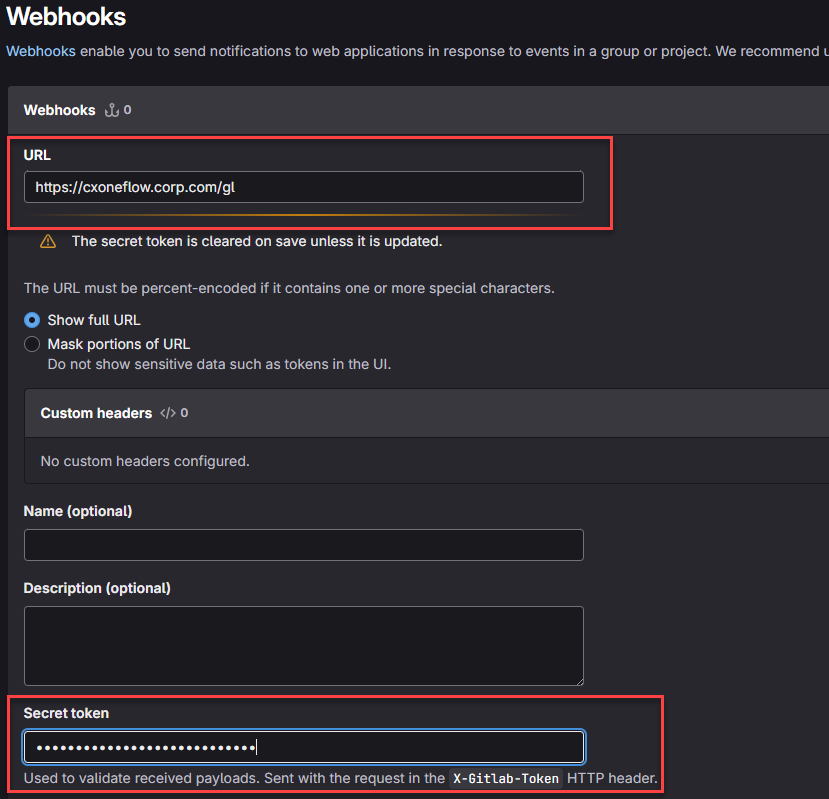
\includegraphics[width=\textwidth]{graphics/gl-project-hook-1.png}
  \caption{Gitlab Group/Project Webhook Endpoint Configuration}
  \label{fig:gl-project-1}
\end{figure}

Figure \ref{fig:gl-project-2} shows the webhook configured to send events for 
\textbf{Push events} and \textbf{Merge request events}.  While it is possible to filter
which branches emit push events, doing so may cause \cxoneflow to not work as expected.

Click the "Add webhook" button to deploy the webhook definition.  Gitlab will immediately start delivering
events to the configured \cxoneflow endpoint.


\begin{figure}[ht]
  \centering
  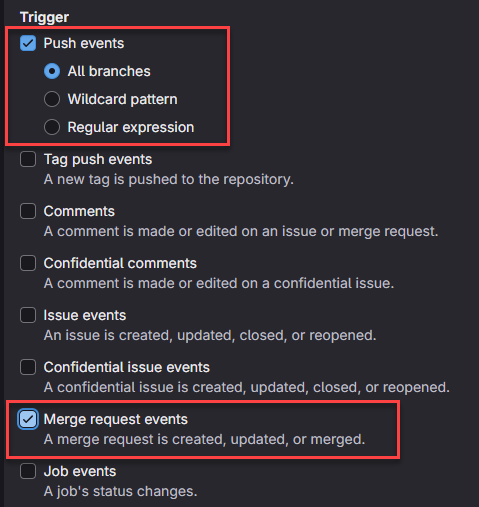
\includegraphics[width=\textwidth]{graphics/gl-project-hook-2.png}
  \caption{Gitlab Group/Project Webhook Event Configuration}
  \label{fig:gl-project-2}
\end{figure}



\section{Protected Branches}

Gitlab allows for a group scope definition of a "default branch" that can be overridden at the
project scope.  The default branch may be considered a protected branch (e.g. it limits who can
commit to the default branch), but Gitlab does not require the default branch to be a protected
branch.  For consistency with \cxoneflow workflow logic with other SCMs, the default branch is
considered a protected branch for all event handling workflows.  This means a push to the 
default branch or a merge request targeting the default branch will initiate a scan regardless
of the configured protection status.

Branch protection rules other than those associated with the default branch can be configured at
the project scope.  The rules allow a named branch to be configured as protected or to supply
a wildcard to protect branches with names that match the wildcard specification.  \cxoneflow will
follow the Gitlab configuration logic for protected branches when handling an event.  Any push
or merge request targeting a protected branch will initiate a scan.



\section{\cxoneflowtext\space YAML Configuration for GitLab}

Below is a listing of a minimal Gitlab YAML configuration.  The elements to note in this
configuration:

\begin{itemize}
    \item The \texttt{base-url} is the root URL for the Gitlab instance.  This URL is also used
    when forming display links such as links to code in PR comments.
    \item The \texttt{api-url-suffix} is the path extension appended to \texttt{base-url} for API requests.
    \item The \texttt{repo-match} regular expression matches the service definition with events emitted by any repository
    in the Gitlab instance.
\end{itemize}

\begin{code}{Minimal YAML Configuration Example}{Gitlab Webhooks}{}
  secret-root-path: /run/secrets
  server-base-url: https://cxoneflow.mydomain.com:8443/
  
  gh:
      - service-name: Gitlab
        repo-match: ^http(s)?:(\/){2}gitlab\.corp\.com.*
        feedback:
          pull-request:
            enabled: True
        connection:
          base-url: https://gitlab.corp.com
          api-url-suffix: api/v4
          shared-secret: scm-shared-secret
          api-auth:
            token: ghe-token
        cxone:
          tenant: mytenant
          oauth:
            client-id: my-oauth-id
            client-secret: my-oauth-secret
          iam-endpoint: US
          api-endpoint: US
\end{code}
    

\section{Deploying Webhook Configurations in Gitlab}

The scope where webhooks are deployed for \cxoneflow will determine how to provision a PAT
that has the appropriate permissions to the projects in the deployment scope.  Using service
hooks, for example, requires a PAT from a user that has access to all projects in the Gitlab
instance.

Deploying webhooks at the project or group scope requires a PAT from a user that has access
to the projects in the deployed scope.  This may require multiple \cxoneflow service definitions
with the \texttt{repo-match} regular expression such that events in the scope available to a
PAT are handled properly.

A PAT, regardless of user or scope, requires the following permissions:

\begin{itemize}
  \item api
  \item api\_read
  \item ai features
\end{itemize}

\subsection{Service Hooks}

A Gitlab administrator can configure system-wide service hooks.  The service hooks configuration is located in the
administrative configuration menu, accessible by clicking the "Admin" button as shown in Figure \ref{fig:gl-admin-menu}.

\begin{figure}[ht]
  \centering
  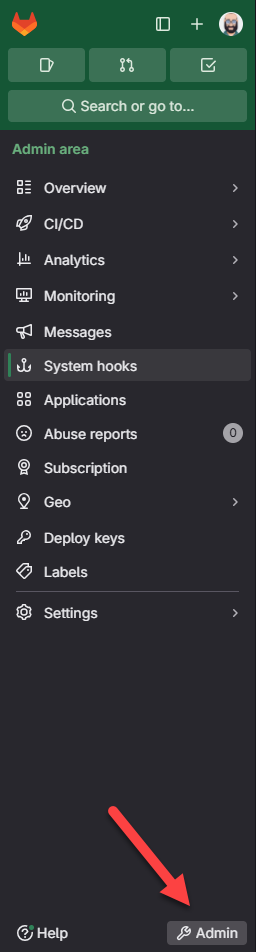
\includegraphics[scale=.5]{graphics/gl-system-hook-admin.png}
  \caption{Gitlab System Hook Administration Menu}
  \label{fig:gl-admin-menu}
\end{figure}


An example service hook definition is shown in Figure \ref{fig:gl-service-hook-def}.  The following are
required configuration elements:

\begin{itemize}
  \item The URL to the \cxoneflow instance ending with the \texttt{gl} route.
  \item The value provided in the \texttt{shared-secret} element under the \texttt{connection} element in the service definition.
  \item The triggers should be \textbf{Push events} and \textbf{Merge request events}.
\end{itemize}

Click the "Add webhook" button to deploy the service hook definition.  Gitlab will immediately start delivering
events to the configured \cxoneflow endpoint.

\begin{figure}[ht]
  \centering
  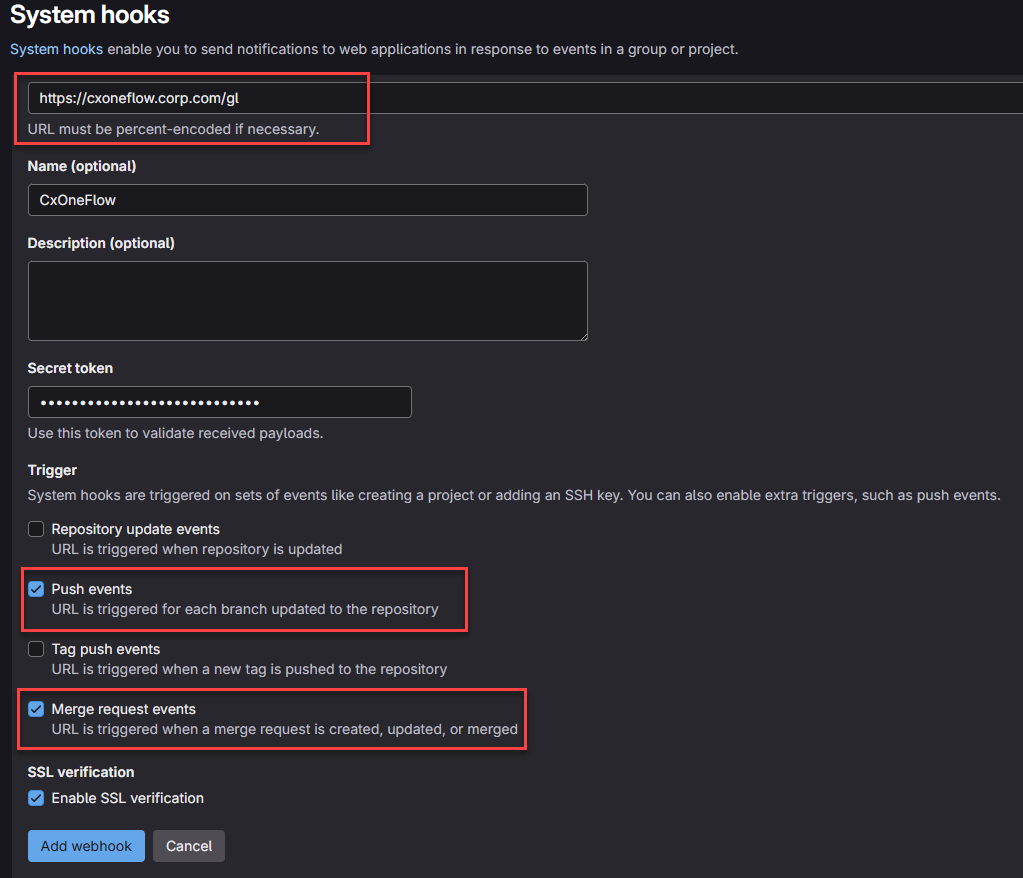
\includegraphics[width=\textwidth]{graphics/gl-service-hooks.png}
  \caption{Gitlab System Hook Definition}
  \label{fig:gl-service-hook-def}
\end{figure}

\subsection{Group or Project Webhooks}

Webhook configurations at the group or project scope operate the same.  The settings for each
are accessed by navigating to the group or project view and selecting \textbf{Settings->Webhooks}.
If attempting to configure webhooks at the group scope in a free Gitlab self-hosted instance or
a free Gitlab cloud account, you will be prompted to purchase a license.

The webhook configuration can be initiated by clicking the \textbf{Add new webhook} button. Figure \ref{fig:gl-project-1}
shows the endpoint configuration where the URL for the \cxoneflow instance with the \texttt{gl} is provided
along with the shared secret.  The shared secret value should match the value provided in the
\texttt{shared-secret} element under the \texttt{connection} element in the service definition.

\begin{figure}[ht]
  \centering
  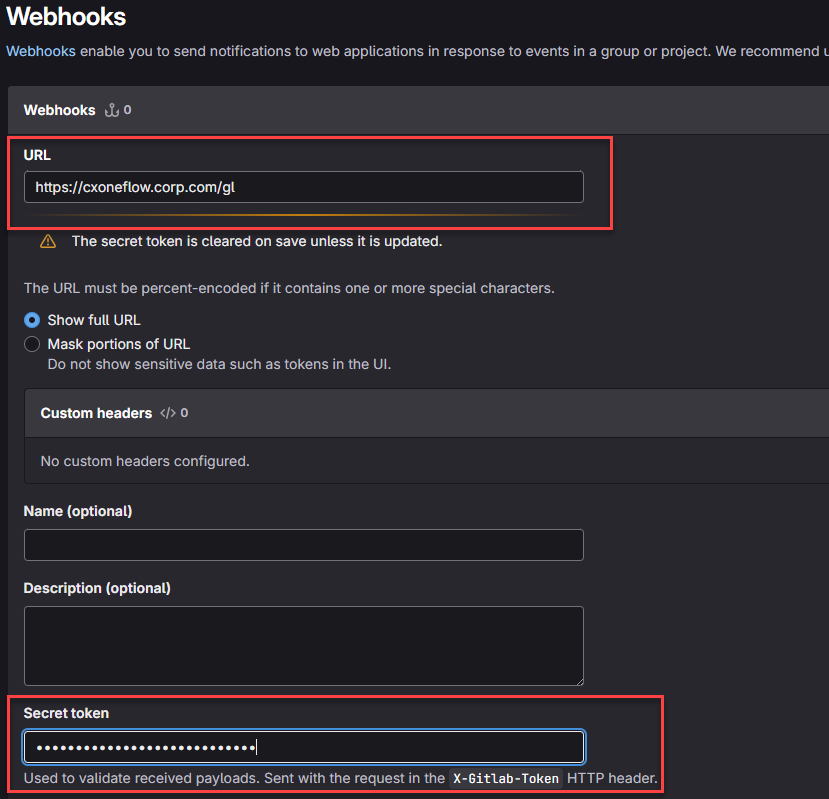
\includegraphics[width=\textwidth]{graphics/gl-project-hook-1.png}
  \caption{Gitlab Group/Project Webhook Endpoint Configuration}
  \label{fig:gl-project-1}
\end{figure}

Figure \ref{fig:gl-project-2} shows the webhook configured to send events for 
\textbf{Push events} and \textbf{Merge request events}.  While it is possible to filter
which branches emit push events, doing so may cause \cxoneflow to not work as expected.

Click the "Add webhook" button to deploy the webhook definition.  Gitlab will immediately start delivering
events to the configured \cxoneflow endpoint.


\begin{figure}[ht]
  \centering
  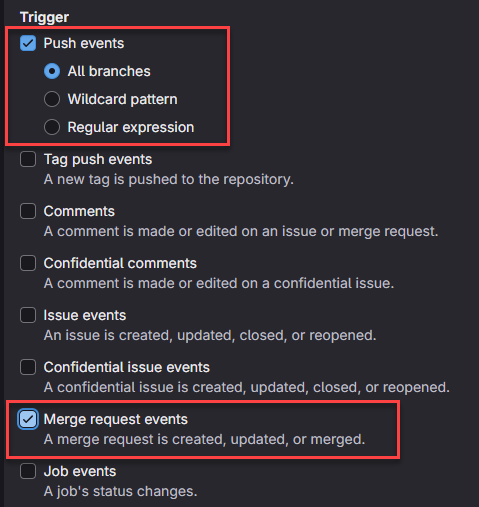
\includegraphics[width=\textwidth]{graphics/gl-project-hook-2.png}
  \caption{Gitlab Group/Project Webhook Event Configuration}
  \label{fig:gl-project-2}
\end{figure}



\section{Protected Branches}

Gitlab allows for a group scope definition of a "default branch" that can be overridden at the
project scope.  The default branch may be considered a protected branch (e.g. it limits who can
commit to the default branch), but Gitlab does not require the default branch to be a protected
branch.  For consistency with \cxoneflow workflow logic with other SCMs, the default branch is
considered a protected branch for all event handling workflows.  This means a push to the 
default branch or a merge request targeting the default branch will initiate a scan regardless
of the configured protection status.

Branch protection rules other than those associated with the default branch can be configured at
the project scope.  The rules allow a named branch to be configured as protected or to supply
a wildcard to protect branches with names that match the wildcard specification.  \cxoneflow will
follow the Gitlab configuration logic for protected branches when handling an event.  Any push
or merge request targeting a protected branch will initiate a scan.


